\documentclass[a4paper,12pt]{article}
\usepackage[utf8]{inputenc}
\usepackage{wrapfig}
\usepackage{graphicx}
\usepackage{float}
\usepackage{amsmath}
\usepackage{pslatex}
\usepackage[portuguese]{babel}
\usepackage{indentfirst}
\usepackage{natbib}
\usepackage[textsize=tiny]{todonotes}
\usepackage{tikz}
\usepackage{url}
\usepackage{hyperref}
\usepackage[lmargin=3cm,rmargin=3cm,tmargin=2.5cm,bmargin=2.5cm]{geometry}
\setlength{\parindent}{1cm}
\setlength{\baselineskip}{1.5cm}

\renewcommand{\contentsname}{Sumário}
\hypersetup{
    bookmarks=false,         % show bookmarks bar?
    unicode=false,          % non-Latin characters in Acrobat’s bookmarks
    pdftoolbar=true,        % show Acroat’s toolbar?
    pdfmenubar=true,        % show Acrobat’s menu?
    pdffitwindow=false,     % window fit to page when opened
    pdfstartview={FitH},    % fits the width of the page to the window
    pdftitle={My title},    % title
    pdfauthor={Author},     % author
    pdfsubject={Subject},   % subject of the document
    pdfcreator={Creator},   % creator of the document
    pdfproducer={Producer}, % producer of the document
    pdfkeywords={keyword1, key2, key3}, % list of keywords
    pdfnewwindow=true,      % links in new PDF window
    colorlinks=true,       % false: boxed links; true: colored links
    linkcolor=blue,          % color of internal links (change box color with linkbordercolor)
    citecolor=blue,        % color of links to bibliography
    filecolor=magenta,      % color of file links
    urlcolor=blue           % color of external links
}


\begin{document}

\begin{titlepage}
 \begin{center}
  { \large FUNDAÇÃO GETULIO VARGAS}\\[0.3cm]
  { \large ESCOLA DE MATEMÁTICA APLICADA}\\[0.5cm]
  { \large CURSO DE GRADUAÇÃO EM}\\[0.3cm]
  { \large MATEMÁTICA APLICADA}\\[0.3cm]
 
  \vspace{55 mm}

  {\bf \large Dinâmica de Disseminação de Notícias em}\\[0.1cm]
  {\bf \large Redes Complexas}\\[1.7cm]

  { por}\\[0.6cm]
  {\large Elisa Mussumeci}\\[0.1cm]


  \vspace{7cm}

  { Rio de Janeiro}\\[0.1cm]
  { 2015}\\[0.6cm]
  { FUNDAÇÃO GETÚLIO}\\[0.1cm]
  { VARGAS}\\[0.1cm]
 \end{center}
\end{titlepage}

\begin{titlepage}
 
 \begin{center}
  {\large FUNDAÇÃO GETULIO VARGAS}\\[0.3cm]
  {\large ESCOLA DE MATEMÁTICA APLICADA}\\[0.5cm]
  {\large CURSO DE GRADUAÇÃO EM}\\[0.3cm]
  {\large MATEMÁTICA APLICADA}\\[0.3cm]


  \vspace{20 mm}


  {\large Dinâmica de Disseminação de Notícias em}\\[0.1cm]
  {\large Redes Complexas}\\[2.5cm]

  
  \bf "Declaro ser o único autor do presente projeto de monografia que refere-se ao
plano de trabalho a ser executado para continuidade da monografia e ressalto
que não recorri a qualquer forma de colaboração ou auxílio de terceiros para
realizá-lo a não ser nos casos e para os fins autorizados pelo professor orientador"

  \vspace{3.5cm}


  \line(1,0){220}\\[0.1cm]
  {\bf Elisa Mussumeci}\\[2cm]
  {\bf Orientador: Flavio Codeço Coelho}\\[5cm]




  {Rio de Janeiro}\\[0.1cm]
  {2015}
 \end{center}
\end{titlepage}

\begin{titlepage}
 \begin{center}
 
  {\bf \large ELISA MUSSUMECI}\\[0.3cm]

  \vspace{25 mm}

  {\bf \large Dinâmica de Disseminação de Notícias em}\\[0.1cm]
  {\bf \large Redes Complexas}\\[4cm]

  {“Monografia apresentada à Escola de Matemática Aplicada}\\[0.1cm]
  {como requisito parcial para obtenção do grau de Bacharel }\\[0.1cm]
  {em Matemática Aplicada”}\\[6cm]


  {Aprovado em \ \line(1,0){20} \ \ de \line(1,0){62} \ \ de \line(1,0){30} \ .}\\[0.1cm]
  {Grau atribuido ao Projeto de Monografia: \line(1,0){20} \ . }\\[3cm]
  
  
  {\line(1,0){250}}\\
  {\bf Professor Orientador: Flávio Codeço Coelho}\\[0.1cm]
  {\bf Escola de Matemática Aplicada}\\[0.1cm]
  {\bf Fundação Getulio Vargas}
 \end{center}
\end{titlepage}

\newpage\null\thispagestyle{empty}\newpage

\tableofcontents

\pagebreak

\listoffigures

\pagebreak

\begin{abstract}
 
O processo de formação de opinião é fortemente influenciado pela mídia digital.
Entretanto pouco se sabe sobre o processo de disseminação de notícias e os fatores que determinam o alcance de cada
notícia.

A disseminação de uma notícia se dá por meio de um ou mais caminhos em uma rede desconhecida de influência entre 
formadores de opinião (produtores de notícias). Este padrão pode ser recuperado, com algum grau de incerteza, a partir de dados
da sequência temporal das publicações sobre um mesmo tema, e dos links nelas contidos.

Este projeto tem como objetivo caracterizar as redes de interligação de veículos de mídia e modelar a dinâmica do espalhamento 
de notícias, a fim de prever tendências e mapear questões de interesse.

\end{abstract}

\pagebreak

\section{Introdução}

Atualmente a internet é um dos principais meios de veiculação de notícias e informação do país. Com o crescente
número de pessoas aderindo à redes sociais, o compartilhamento de notícias aumentou significamente, o que tornou fundamental
o papel das mídias digitais no acesso à informação.

Consideramos como mídia digital todo e qualquer veículo difusor de informação contido na internet brasileira, como jornais, revistas e 
blogs independentes. Cada mídia presente na internet possui sua própria periodicidade, alcance, público e credibilidade, o que afeta
diretamento no processo de disseminação da informação.

Utilizando do fato que essas mídias digitais são fundamentais na disseminação da informação, e que com isso possuem um forte papel 
influenciador no processo de formação de opinião, podemos definir como importante entender como as notícias se formam e se espalham
na internet brasileira.

Um dos métodos de se estudar a disseminação da informação é utilizando modelos epidemiológicos. \cite{bettencourt2006power} conseguiu modelar a disseminação de (tabela de alguma coisa) no tempo através de modelos epidemiológicos, como SIR, SIS entre outros. Ese tipo
de abordagem vem sendo utilizada também para entender redes de contatos em redes sociais como (incluir referencia). MELHORAR PARAGRAFO

Neste trabalho utilizaremos redes complexas e modelos epidemiológicos para modelar a disseminação de notícias na mídia brasileira. 
Para isso
estudaremos os caminhos percorridos em uma rede de disseminação criada através de modelos de recuperação de informação utilizados em cima
da base de dados do Projeto MediaCloud Brasil\footnote[1]{\url{https://github.com/NAMD/mediacloud_backend}}.


\subsection{O Projeto Media Cloud Brasil}

 O MediaCloud Brasil é um projeto concebido através de uma parceria do NAMD/EMAp da Fundação Getúlio Vargas, do Massachussets Institute of
 Technology (MIT)  e Harvard. O projeto

 e mantido pelo NAMD/EMAp da Fundação Getúlio Vargas, e vem ao longo dos últimos três anos 
 monitorando mais de cem mil veículos de mídia da internet brasileira. 
 O projeto consiste na captura automatizada de dados de tods of feeds da mídia digital brasileira, captura-se páginas de blogs, jornais, revistas,
 
 Possui em
sua base de dados mais de 1.6 milhão de artigos capturados.
\textbf{falar sobre o que e como o Media cloud captura os artigos}
O projeto utiliza como banco de dados o MongoDB, um banco de dados de documentos open-source de alta performance. O MongoDB é classificado como um banco de 
dados 'NoSQL', uma vez que evita a tradicional estrutura  baseada em tabela relacional e utiliza documentos JSON com esquemas dinâmicos para armazenamento 
dos documentos. A vantagem de utilizar o JSON é realizar a integração de dados em certos tipos de aplicações de forma mais fácil e mais rápida.\todo{Que tipo de aplicações?}
\textbf{Falar que uma vez armazenado, o banco de artigos é indexado para permitir buscas textuais}

\subsection{Referencial Teórico}


\subsubsection{O espalhamento de notícias como um processo de contágio}

Uma epidemia é caracterizada pela incidência de grande número de casos de uma doença em um curto período de tempo. Sabemos que as doenças
se espalham através do contágio entre infectados, mas como podemos definir esse contágio? 

Cada doença possui uma forma própria de transmissão, por exemplo, a gripe é uma doença viral e se transmite a partir de vias orais, já a dengue
é transmitida a partir da picada de um mosquisto, assim como a febre amarela. Saber a forma de contágio de uma doença é fundamental para que
possamos entender sua disseminação e modelar sua epidemia.

Ao observar o comportamento de notícias, assuntos e histórias na mídia, podemos ver o surgimento de memes e histórias 'virais'. Esses 
tipos de notícias são chamadas de virais por se espalharem muito rápido e obterem um alcançe grande na população. Algumas dessas notícias
se sustentam por um longo tempo na mídia, e outras são esquecidas rapidamente. 

Se pensarmos que estamos lidando com um processo de disseminação, que possui uma taxa de espalhamento e uma taxa de esquecimento, podemos
facilmente fazer uma comparação à modelos epidemiológicos, principalmente ao modelo SIR, que possui uma taxa de infecção e
uma taxa de recuperação. Dessa forma, podemos estudar como uma notícia se espalha da mesma forma que modelamos uma epidemia.

Para modelar a disseminação de notícias da mesma forma que modelamos a de doenças, precisamos
que nosso modelo seja compatível com o de uma epidemia, ou seja, precisamos definir os infectados, suscetíveis e o método de contágio.

Em nosso modelo, uma notícia/assunto é a doença, e os infectados são todos os artigos que falam sobre essa notícia. 
Para definir o contágio da nossa notícia, consideramos que um artigo infecta o outro quando ele influência o outro. Ou seja,
definimos que quando um artigo exerceu influência sobre um outro, ele infectou esse outro artigo. 

Dessa forma, podemos ver a similaridade entre ambas modelagens, o que deixa claro a possibilidade de modelar a disseminação de
notícias através de modelos epidemiológicos. O que nos falta descobrir são os parâmetros que utilizaremos para realizar essa modelagem
de forma que fique o mais verídica possível.

\subsubsection{Processos Epidemiológicos em Redes Complexas}

 O termo Redes Complexas se refere a um grafo que apresenta uma estrutura topográfica não trivial, composto por um conjunto
 de vértices (nós) que são interligados por meio de arestas (\cite{ravasz2003hierarchical}). A teoria das Redes Complexas  
 está relacionada com a modelagem de redes reais, através da 
 análise de dados empíricos. As redes complexas não são estáticas (evoluem no tempo alterando sua estrutura), e 
 constituem estruturas onde processos dinâmicos (como disseminação de virus ou opiniões) podem ser simulados.
 
 Um processo dinâmico comumente modelado como rede complexa é a disseminação de uma doença na população. Através da rede
 conseguimos observar o processo de infecção dinâmicamente, e realizar análises que trazem resutados significativos para o modelo epidemico,
 como estudar os caminhos percorridos e definir parâmetros de infecciosidade.
 
 
\subsubsection{Processamento de Linguagem Natural}
\label{sec:nlp}

Processamento de Linguagem Natural \textit{(Natural Process Lenguage - NLP)} é uma área de Inteligência Artifical que tem como principal
objetivo desenvolver métodos computacionais que consigam traduzir a linguagem natural para a máquina. A utilização desses
métodos é fundamental em tarefas que envolvem análises conjuntos de dados, pois a partir deles podemos
traduzir os textos para uma linguagem compreensivel ao computador.

\begin{description}
  \item \textbf{Pré-Processamento}
  
    O primeirio passo ao lidar com documentos em texto em computadores é realizar um pré-processamento no conjunto de dados. Esse 
    pré-processamento consiste em  tokenizar, limpar e stemmatizar cada documento do corpus linguístico. 
    
    O processo de tokenização consiste em decompor o documento em termos, também chamado de  tokens. Para cada documento, cria-se uma lista de 
    tokens presentes nele. Após tokenizar, limpamos o documento retirando  as \textit{stop-words} (lista de termos não representativos para
    documentos, geralmente composta por preposições, pronomes, pontuação, advérbios e artigos) e realizamos o processo de 
    \textit{stemming}, que consiste em radicalizar cada termo do documento. Dessa forma, palavras que possuem o menos radical são consideradas
    iguais, já que representam a mesma definição.
    
    Temos como exemplo as duas frases a seguir:
    
    \begin{center}
      \begin{enumerate}
	\item João gosta de jogar futebol. Maria prefere jogar xadrez.
	\item Maria não gosta de futebol.
      \end{enumerate}
    \end{center}
    

    Após o pré-processamento temos:
    
    \begin{center}
      \begin{enumerate}
	\item (joão, gost, jog, futebol, maria, prefer, jog, xadrez)
	\item (maria, não, gost, futebol)
      \end{enumerate}
    \end{center}
    
    
  \item \textbf{Bag-of-Words}
  
   O modelo bag-of-words é uma forma de representar vetorialmente um texto muito usada em Processamento de Linguagem Natural e em
   Recuperação de Informação. O modelo consiste em aprender um vocabulário baseado em todos
   os documentos pré processados do conjunto de dados, e então modelar o documento a partir número de vezes em que
   cada palavra do vacabulário aparece. Dessa forma, cada documento é representado por um 'saco de palavras', o que, apesar de manter
   multiplicadade, causa uma perda de informação, visto que não leva em consideração a ordem  e posição das palavras.
   
   Exemplifcamos o proocesso a seguir, considerando as frases pré processadas na seção anterior:
   
    \begin{center}
      \begin{enumerate}
	\item (joão, gost, jog, futebol, maria, prefer, jog, xadrez)
	\item (maria, não, gost, futebol)
      \end{enumerate}
    \end{center}
    
    Cria-se então o vocabulário do conjunto de dados:
    
   \begin{center}
    \{joão, gost, jog, futebol, maria, prefer, xadrez, não\}
   \end{center}

   A partir desse vocabulário, criamos então, o vetor referente a cada palavra:

    \begin{center}
      \begin{enumerate}
	\item (1,1,2,1,1,1,1,0)
	\item (0,1,0,1,1,0,0,1)
      \end{enumerate}
    \end{center}
   
 
 \item \textbf{Skip-gram}

  O \textit{Skip-gram} é um modelo deep-learning que tem como objetivo representar palavras com o maior valor semântico possível, ou seja
  uma representação que leva em consideração o contexto. Intruduzido
  por \cite{mikolov2013efficient}, o skip-gram é uma rede neural que ao treinar um corpus linguístico, retorna para cada palavra um vetor 
  representativo de atributos.
  
  A maior vantagem desse modelo é que palavras semelhantes possuem vetores próximos no espaço, ou seja, atráves dos atributos calculados pelo
  modelo conseguimos definir a semelhança semântica entre duas palavras. Esse fator faz do skip-gram um modelo essencial para este trabalho
  que tem na semelhança entre textos uma de suas principais eurísticas.
  
 \item \textbf{TF-IDF}
 
  O modelo Tf-Idf (\textit{term frequency-inverse document frequency}), é uma medida estatística que tem o intuito de indicar
  a importância de uma palavra de um documento em relação a um corpus linguístico. O Tf-Idf é definido através do produto entre as 
  estatísticas $Tf_{d,t}$ e $Idf_{t}$.

  Dado um conjunto de $N$ documentos, $Tf_{d,t}$ é a frequência do termo $t$ no documento
  $d$, ou seja, o número de vezes em que $t$ ocorre em $d$. Sendo assim, o $Tf$ nos dá a frequência absoluta dos termos, 
  o que faz com que um termo que possui frequência alta seja relevante.
  
  O termo $Idf_{t}$ tem como função aumentar o peso relativo de termos raros e diminuir o peso relativo de termos muito frequentes,
  uma vez que termos raros são mais informativos do que termos frequentes. Calculamos a medida TF-IDF $ W_{t,d}$ do termo $t$ no documento
  $d$ da seguinte forma:

  $$ W_{t,d} = (1 + log Tf_{t,d}) \cdot \ log \dfrac{N}{Df_{t}}$$

  Onde $Df_{t}$ é uma medida inversa da informatividade do termo $t$, e é definida como o número de documentos em que $t$ ocorre. O peso
  TF-IDF aumenta com o número de ocorrências dentro de um documento e com a raridade do termo na coleção.
\end{description}

\subsection{Objetivo}

Esse trabalho tem como principal objetivo caracterizar e modelar a dinâmica de disseminação das notícias no país através de redes complexas.




\pagebreak
\section{Metodologia}

\subsection{Rede de Disseminação Real}

Nesta primeira parte do trabalho, iremos construir uma rede complexa que descreva o processo epidemiológico de uma notícia. O objetivo
da construção dessa rede, é conseguir aproximar a rede de interligação real entre os artigos selecionados do banco
MediaCloud, de forma a torná-la observável.

Primeiramente, selecionamos todos os artigos do banco referentes a uma determinada notícia, criando assim, nosso corpus linguístico.
Depois ,a partir desse corpus, utlizamos métodos de PLN para representar matricialmente nosso conjunto de dados. A partir da matriz 
criada construímos nossa rede direcionada de disseminação, onde cada vértice ou nó da rede é um artigo.

Para construir a rede de disseminação precisamos definir a relação de contágio entre artigos, ou seja, o que conecta um artigo ao outro 
na rede. No nosso caso, definimos que o contágio se dá através de uma relação de influência, porém como definir essa relação? Partindo do
pressuposto de que se um artigo influênciou outro então esses artigos são necessariamente similares, consideramos a \textbf{similaridade}
entre os artigos o fator principal para definir se eles possuem uma conexão em nossa rede.

Possuindo uma conexão, ainda precisamos saber quem influênciou e quem foi o influenciado. Para definir isso, utilizamos o \textbf{tempo}.
Assim, dado que dois artigos são similares, definimos como influenciador o artigo que fui publicado primeiro e influenciado o artigo publicado
depois. No caso de um artigo ter mais de um similar publicado anteriormente a ele, definimos como influenciador o artigo
mais similar à ele. Dessa forma todos os vértices de nossa rede possuem um grau de entrada igual à 1 e podem possuir um grau de saída maior
do que 1.

A seguir, podemos ver um exemplo do que esperamos da nossa rede de disseminação real:


\begin{figure}[h]
 \centering
 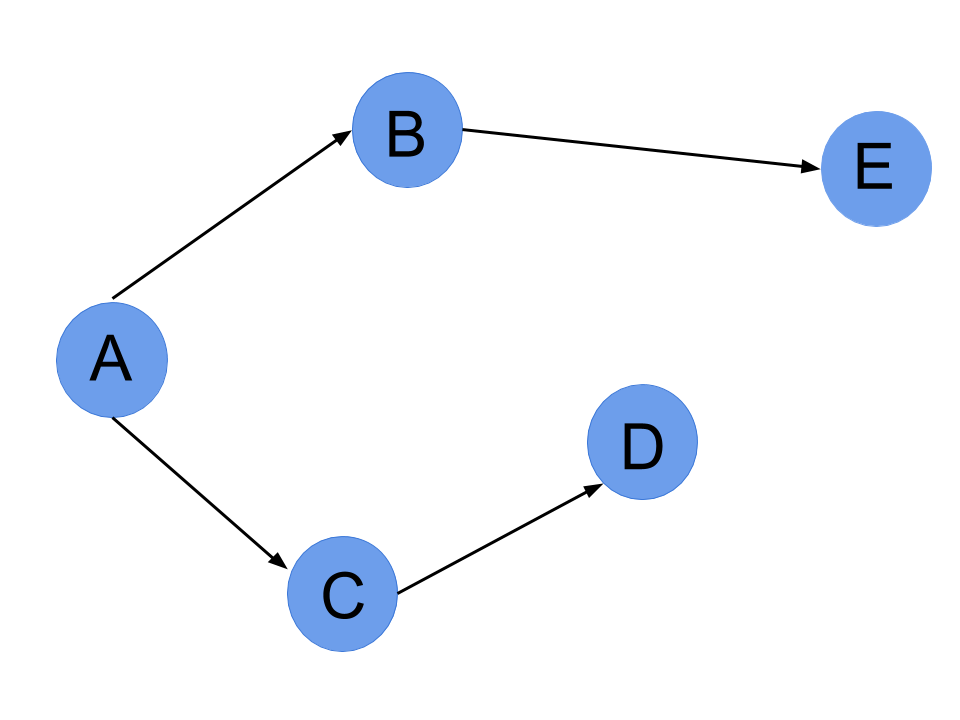
\includegraphics[scale=0.2]{./rede1.png}
 % rede1.png: 960x720 pixel, 72dpi, 33.87x25.40 cm, bb=0 0 960 720
 \caption{Rede Real Genérica}
\end{figure}

No exemplo acima, temos que o artigo $A$ é similar aos artigos $B$ e $C$ e possui uma data de publicação mais antiga do que os dois. 
Sendo assim, foi definido como o influenciador dos dois, ou seja, foi o artigo que os contagiou com a notícia.

\pagebreak
\subsubsection{Matriz de Documentos}

Selecionamos no banco de dados do MediaCloud todos os artigos referentes a uma determinada notícia, formando o corpus linguístico que 
utilizaremos para criar a matriz de documentos, representação vetorial dos artigos selecionados.

Para representar vetorialmente nosso conjunto de dados utilizamos o \textit{Word2Vec}\footnote[1]{\url{https://code.google.com/p/word2vec/}}, ferramenta que promove uma implementação 
eficiente do modelo \hyperref[sec:nlp]{skip-gram} e \hyperref[sec:nlp]{bag-of-words} contínuo.\todo{preciso explicar mais sobre o word2vec?}

Para gerar nosso modelo Word2Vec \todo{preciso explicar que tem que haver um conjunt trainado com todos os artigos do mediacloud etcs?}, fornecemos como entrada nosso corpus linguístico
e o modelo nos retorna uma matriz, onde as linhas $p_{1},p_{2},...,p_{n}$ são as palavras contidas no corpus e as colunas $t_{1},t_{2},...,t_{n}$
são os atributos gerados pelo modelo para cada palavra:
 
 \begin{center}
 \hspace{0.2cm}$t_{1}$ \hspace{0.5cm} $t_{2}$ \hspace{0.3cm} $\hdots$ \hspace{0.4cm}$t_{n}$
 
 \vspace{0.2cm}
 
\begin{tabular}{c}
   $p_{1}$ \\
   $p_{2}$ \\
   \vdots\\
   $p_{n}$
 \end{tabular}
 $
 \begin{bmatrix}
  a_{11} & a_{12} & \hdots & a_{1n}\\
  a_{21} & a_{22} & \hdots & a_{2n}\\
  \vdots & \vdots & \ddots & \vdots\\
  a_{31} & a_{32} & \hdots & a_{nn}
 \end{bmatrix}_{nxn}
$

\end{center}

Dessa forma, temos uma matriz de palavras, ou seja, uma representação de todas as palavras presentes em nosso corpus.
Porém, queremos representar documentos e não apenas palavras.
Para criar uma matriz que represente documentos, fazemos, para cada documento, uma soma dos vetores referentes a cada palavra presente
no documento, criando assim um vetor representativo do documento em questão.

Podemos exemplificar da seguinte forma: dado um documento $D$, sabemos que ele é composto pelo seguinte conjunto de palavras
$P:\{1,2,3,4,5\}$. Para cada termo, buscamos o seu vetor representativo $p_{i}$, $i =\{1,2,3,4,5\}$ na matriz de
palavras e somamo-os, criando o vetor $v_{D}$ que representa o vetor referente ao documento $D$:

\begin{equation}
  v_{D} = p_{1}+p_{2}+p_{3}+p_{4}+p_{5}
\end{equation}


Ao representar um documento dessa forma, não levamos em consideração a relevância de cada palavra para o documento, o que
faz da nossa representação pouco eficiente. Para melhorar nossa 
eficiência, antes de somar os vetores de palavras $p_{i}$, iremos multiplicar cada um deles pelo valor \hyperref[sec:nlp]{TF-IDF} da palavra
ao qual ele representa.

Sendo assim, sabendo que para cada palavra $i$ temos um vetor $p_{i}$ que a representa na matriz de palavras, e um valor $w_{i,d}$ referente
ao valor \textit{TF-IDF} da palavra $i$ no documento $D$, representamos o vetor $v_{D}$ da seguinte forma:

\begin{equation}
  v_{D} = \sum_{i=1}^{5} p_{i} \cdot w_{t,D}
\end{equation}


Sendo assim, ficamos com a matriz de documentos abaixo, onde cada linha $v_{i}$ é um documento, e cada coluna $t_{i}$ é a soma do atributo $i$
em todas as palavras do documento $i$:

 \begin{center}
 \hspace{0.2cm}$t_{1}$ \hspace{0.5cm} $t_{2}$ \hspace{0.3cm} $\hdots$ \hspace{0.4cm}$t_{n}$
 
 \vspace{0.2cm}
 
\begin{tabular}{c}
   $v_{1}$ \\
   $v_{2}$ \\
   \vdots\\
   $v_{n}$
 \end{tabular}
 $
 \begin{bmatrix}
  a_{11} & a_{12} & \hdots & a_{1n}\\
  a_{21} & a_{22} & \hdots & a_{2n}\\
  \vdots & \vdots & \ddots & \vdots\\
  a_{31} & a_{32} & \hdots & a_{nn}
 \end{bmatrix}_{nxn}
$

\end{center}



\subsubsection{Construção da Rede}

 Construimos a rede de disseminação a partir da matriz de documentos gerada na sessão anterior, onde cada vetor consiste em um documento/artigo.
 
 Ao construir a rede dos nossos documentos,
 consideramos como contágio sofrer influência de outro artigo, ou seja, um artigo A contamina um artigo B se o artigo A influenciou o
 artigo B.
 
 Dessa forma, em nossa rede, os vértices representam os artigos, e as arestas a relação de influência entre eles, isto é, dado um nó $e_{i}$ e um nó
 $e_{j}$, existe uma aresta $a_{ij}$, que sai de \textit{i} e vai para \textit{j}, se o artigo \textit{i} influênciou o artigo \textit{j}.
 
 Para definir quando um artigo influência outro em nossa rede, foram usadas duas heurísticas: \textit{similaridade} e 
 \textit{temporalidade}.
 
 \begin{description}
  \item \textbf{Similaridade}
  
    Para definir similaride entre dois artigos, utilizamos a \textit{Similaridade de Cosseno}. A similaridade de cosseno mede a semelhança entre
    dois vetores através da distância de cosseno do ângulo que eles formam. Para calcular a distância de cosseno $d(A,B)$ entre um vetor $A$ e $B$, fazemos:
    
    \begin{equation}
      d(A,B) = cos(\theta) = \dfrac{A \cdot B}{\parallel A\parallel \parallel B \parallel}
    \end{equation}

    
    A similaridade de cosseno se dá por $1-d(A,B)$.Utilizando essa equação, calculamos a similaridade de cosseno para cada
    par de vetor de nossa matriz de documentos, criando assim, uma matriz de similaridades. Se similaridade entre dois vetores for 
    grande o suficiente, os definimos como similares. 
    
    Para saber o quão grande a similaridade de cosseno entre dois artigos deve ser para considerarmo-os similares, fazemos a
    distribução das similaridade e realizamos um corte em suas extremidades.
    
    
  \item \textbf{Temporalidade}
  
    Após definir dois artigos como similares, inferimos uma relação de influência entre eles. Porém, ainda precisamos saber quem influeciou e quem
    foi influenciado. Para descobrir isso, olhamos a data de publicação de cada artigo. Se dois artigos $A$ e $B$ foram considerados 
    similares, e o artigo $A$ foi publicado antes do artigo $B$, então definimos que $A$ influenciou $B$, logo temos em nossa rede:
    
    \begin{figure}[h]
      \centering
      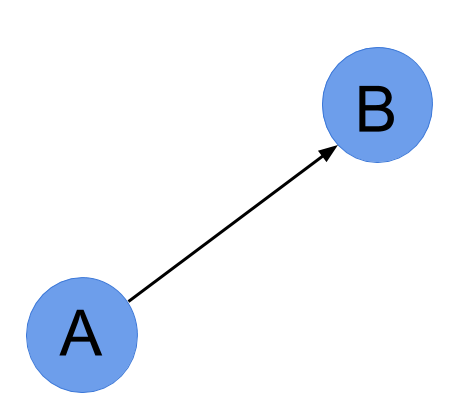
\includegraphics[scale=0.2]{./rede2.png}
      % rede2.png: 960x720 pixel, 72dpi, 33.87x25.40 cm, bb=0 0 960 720
      \caption{Relação de Influência}
    \end{figure}
    
    \pagebreak

    Porém, pode acontecer de termos um outro artigo $C$, também considerado similar ao artigo $B$ e que também publicado anteriormente. Em nosso modelo,
    definimos que um artigo só pode ter sido influênciado por um único artigo. Dessa forma, como definir quem de fato influênciou $B$? Para
    resolver esse impasse utilizamos a similaridade de cosseno. Consideramos influênciador o artigo publicado anteriormente, e que possui
    a \textbf{maior} similaridade com $B$.
    
    Consideramos, também, que um artigo deixa de ser influente com o passar do tempo, assim como uma pessoa infectada por um vírus deixa
    de ser infecciosa após se curar da doença. Dessa forma, precisamos calcular o tempo máximo em que um artigo é influente em nossa rede.
    Para isso, calculamos a diferença entre as datas de publicação de cada par de artigos e fazemos a distribuição dessas diferenças. Assim como
    na distribuição de similaridades, realizamos um corte nas extremidades e pegamos os valores limites.
 \end{description}
 

\subsection{Simulação Rede de Disseminação}

Na segunda parte do trabalho, temos como objetivo simular a disseminação de nossa rede real utilizando um modelo epidemiológico, com o intuito
de validarmos nossa rede e conseguirmos caracterizá-la.

Queremos então, conseguir modelar a disseminação de uma notícia em uma rede genérica e conseguir um resultado semelhante à nossa rede de
disseminação real. Dessa forma, dado uma rede completa com $N$ nós, queremos traçar o espalhamento da infecção nesses $N$ nós, ou seja, definir
as relações de influencia entre eles, utilizando os resultados de uma simulação epidemiológica:
\vspace{0.4cm}

\begin{figure}[ht]
\centering
\begin{minipage}{.5\textwidth}
  \centering
  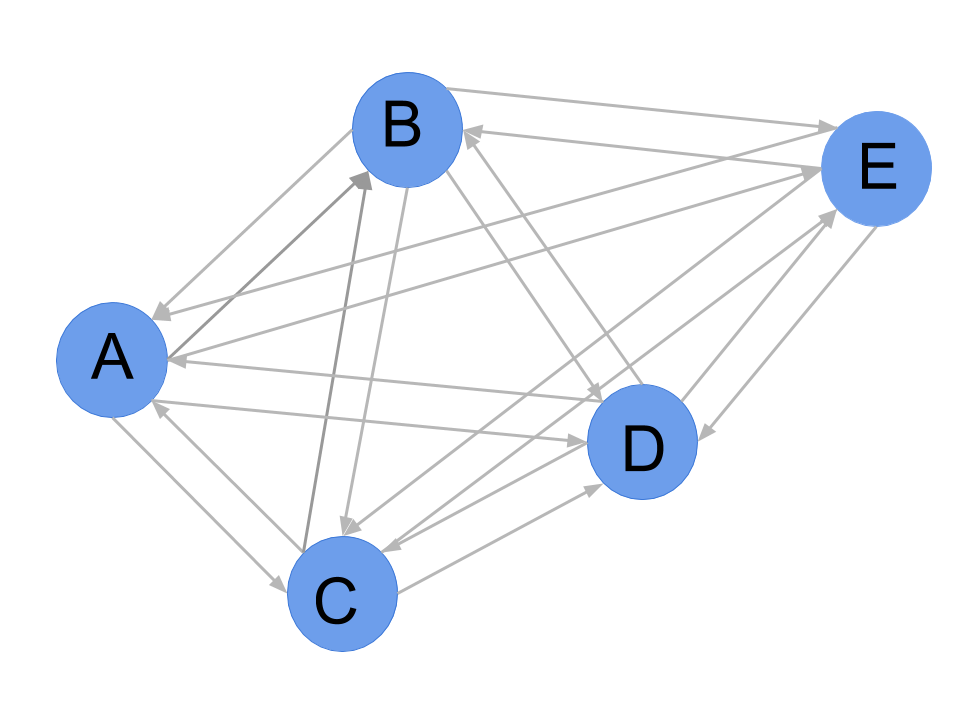
\includegraphics[width=.9\linewidth]{./rede3.png}
  \caption{Rede Completa}
  \label{fig:test1}
\end{minipage}%
\begin{minipage}{.5\textwidth}
  \centering
  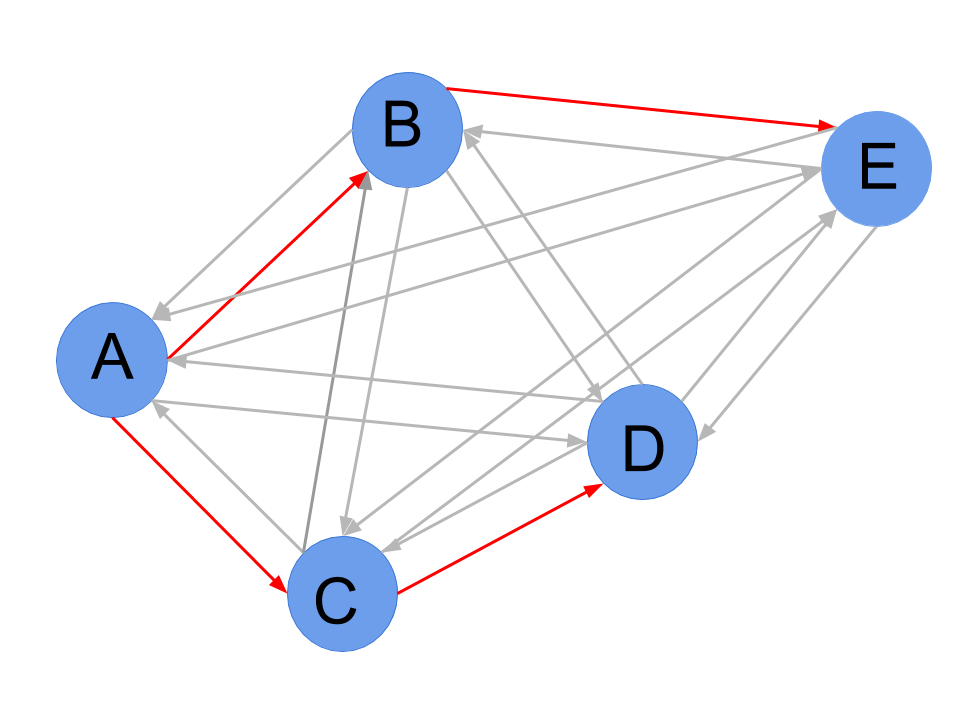
\includegraphics[width=.9\linewidth]{./rede4.png}
  \caption{Disseminação na Rede Completa}
  \label{fig:test2}
\end{minipage}
\end{figure}


\pagebreak
\subsubsection{Criação Rede Completa}


 Para simular nossa rede, construimos primeiramente uma rede completa com os mesmos nós de nossa rede real, onde os pesos das arestas
 são as probabilidades dessa aresta existir no caminho de disseminação da notícia, ou seja, a probabilidade de um artigo influenciar um 
 outro. Podemos exemplificar da seguinte forma, dado duas vértices de nossa rede completa, $A$ e $B$. Teremos como peso para as duas 
 arestas que conectam esses nós a probabilidade de cada uma existir:
 
 \begin{figure}[ht]
 \centering
 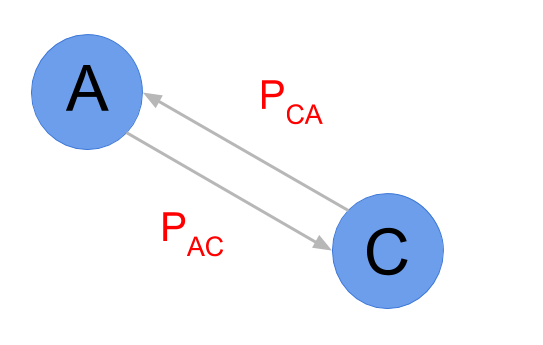
\includegraphics[scale=0.3]{./rede5.png}
 % rede5.png: 543x345 pixel, 72dpi, 19.16x12.17 cm, bb=0 0 543 345
 \caption{Pesos na Rede Completa}
\end{figure}

 Onde $P_{CA}$ e $P_{AC}$ são as probabilidades do nó $C$ ter influenciado o nó $A$, e do no $A$ ter influenciado o nó $C$, 
 respectivamente.

 Calculamos essas probabilidades através da infomação do \textbf{veículo} responsável por cada artigo. Para cada nó presente em nossa rede completa,
 buscamos o veículo que publicou o artigo referente ao nó (exemplos de veículos são oglobo.com, folha.com.br). Possuindo o veículo de cada
 nó presente na rede, podemos saber qual a chance de um artigo do veículo $X$ ser influenciado por um artigo do veículo $Y$. Dessa forma, 
 considerando $X$ e $Y$, os veículos dos nós $A$ e $C$, respectivamente, calculamos a probabilidade $P_{AC}$ da seguinte forma:
 
 \begin{equation}
  P_{AC} = \dfrac{N_{XY}}{NY}
 \end{equation}

 
 Onde  $N_{XY}$ é o número de vezes que um artigo do veículo $X$ influenciou um artigo do veículo $Y$, e $NY$ represnta o número de vezes
 em que um artigo do veículo $Y$ foi influenciado em nossa rede de disseminação real.

 Construímos então uma matriz de pesos, onde calculamos as probabilidades para cada par de veículos. É esperado em um conjunto de 
 dados possuirmos mais de um artigo publicado pelo mesmo veículo, sendo assim, considerando que temos $n$ artigos em nosso corpus 
 linguístico, possuimos nele $m$ veículos responsáveis pela publicação desses $n$ artigos.

 Dessa forma, nossa matriz de pesos possui tamanho $mxm$, e cada posição $a_{ij}$ temos a probabilidade do veículo 
 $i$ ser influenciado pelo veículo $j$. Considerando que um veículo não influencia a si mesmo, teremos a matriz a seguir:
 
 \begin{center}
 \hspace{0.2cm}x \hspace{0.5cm} y \hspace{0.3cm} $\hdots$ \hspace{0.4cm}z
 
 \vspace{0.2cm}
 $
 \begin{tabular}{c}
   x \\
   y \\
   \vdots\\
   z
 \end{tabular}
$
 $
 \begin{bmatrix}
  0 & a_{12} & \hdots & a_{1m}\\
  a_{21} & 0 & \hdots & a_{2m}\\
  \vdots & \vdots & \ddots & \vdots\\
  a_{31} & a_{32} & \hdots & 0
 \end{bmatrix}_{mxm}
$

\end{center}

\vspace{0.4cm}

Utilizando a matriz de pesos acima, atribuiremos os valores para cada aresta de a rede completa criada acima. Para isso, criamos uma matriz
de adjacência, onde cada valor $a_{ij}$, contém a probabilidade dessa aresta existir.
Sendo assim, para cada par de artigos $d_{i},d_{j}$ de nossa rede completa,
descobrimos seus veículos $x$ e $y$, e buscamos a probabilidade de conexão entre eles na matriz de pesos. Dessa forma,
ficamos com uma matriz $nxn$ documentos, que descreve a probabilidade da conexão entre cada par de vértices da rede completa, e que será
essencial para a simualação da disseminação da notícia na rede.
  
 \begin{center}
 \hspace{0.2cm}$d_{1}$ \hspace{0.5cm} $d_{2}$ \hspace{0.3cm} $\hdots$ \hspace{0.4cm}$d_{n}$
 
 \vspace{0.2cm}
 
 \begin{tabular}{c}
   $d_{1}$ \\
   $d_{2}$ \\
   \vdots\\
   $d_{n}$
 \end{tabular}
 $
 \begin{bmatrix}
  0 & a_{12} & \hdots & a_{1n}\\
  a_{21} & 0 & \hdots & a_{2n}\\
  \vdots & \vdots & \ddots & \vdots\\
  a_{31} & a_{32} & \hdots & 0
 \end{bmatrix}_{nxn}
$

\end{center}

\subsubsection{Simulação}

Nesta seção, iremos simular a disseminação da notícia em nossa rede completa. Para isso, simularemos um modelo epidemiológico de forma
que possamos obter o estado de nossa rede em cada passo de contágio, ou seja, queremos saber quais artigos foram infectados em cada passo
$q$ de nossa simulação, e quais artigos foram responsáveis por infectá-los.

 \begin{description}
  \item \textbf{Modelo utilizado}
  
  \todo{não sei o quanto preciso explicar com minas palavras do modelo, talvez tenha ficado meio confuso}
    
    O modelo epidemiológico que iremos simular foi proposto por \citet[p. 940, eq. (33)]{pastor2014epidemic}. Nele,
    simulamos a probabilidade $\rho^{I}_{i}(t)$ de cada artigo $i$ estar infectado em um tempo $t$ utilizando a matriz de adjacência criada na seção anterior:

    \begin{equation}
      \dfrac{d\rho^{I}_{i}}{dt} = -\rho^{I}_{i}(t) + \lambda[1- \rho_{i}^{I}(t)] \sum_{j=1}^{N} a_{ij}\rho_{j}^{I}(t)
      \label{model}
    \end{equation}

    Nossa matriz de adjacências é iterada para cada artigo $i$, como podemos ver no fator $\sum_{j=1}^{N} a_{ij}\rho_{j}^{I}(t)$ da 
    equação diferencial acima. Nela, somamos as probabilidades de cada artigo $j$ ter influenciado o artigo $i$ em questão, vezes a probabilidade
    de cada artigo $j$ estar infectado no tempo $t$, ou seja, a chance de um artigo ja infectado ter infectado o artigo $i$.
    
    Multiplicamos esse resultado pela taxa de transmissão $\lambda$ e pela possibilidade dele ainda não estar infectado (proporção
    de documentos não infectados). Assim obtemos a probabilidade do artigo $i$ se infectar. 
    
    O parâmetro $\lambda$ é obtido através da divisão da taxa de infecção $\beta$ pela taxa de recuperação $\mu$:
    
    \begin{equation}
     \lambda = \dfrac{\beta}{\mu}
    \end{equation}
    
    A equação (\ref{model}) teve o tempo reescaldo em $\dfrac{1}{\mu}$, o que torna nosso modelo adimensional,
    como explicado em \citet[p. 939]{pastor2014epidemic}. Podemos interpretar que o tempo de cada passo é o inverso do tempo de 
    recuperação  média dos artigo. 
   
    Para tornar o resultado da simulação mais fiel ao nosso conjunto de dados, onde possuimos um decaimento da infecção, ou seja,
    nosso artigos se recuperam (deixam de ser influentes), incrementamos a equação abaixo ao modelo:
    
    \begin{equation}
      \dfrac{d\rho^{S}_{i}}{dt} = - \lambda\rho_{i}^{S}(t) \sum_{j=1}^{N} a_{ij}\rho_{j}^{I}(t)
      \label{model2}
    \end{equation}
    
    Essa equação nos diz que um artigo que já foi infectado não pode ser infectado novamente. Modificando o modelo para o incremento
    da equação (\ref{model2}), ficamos com um modelo final utilizado nas simulações:
    
   
    \begin{equation}
      \begin{cases}
	\dfrac{d\rho^{I}_{i}}{dt} = -\rho^{I}_{i}(t) + \lambda\rho_{i}^{S}(t) \sum_{j=1}^{N} a_{ij}\rho_{j}^{I}(t) \\   
	\dfrac{d\rho^{S}_{i}}{dt} = - \lambda\rho_{i}^{S}(t) \sum_{j=1}^{N} a_{ij}\rho_{j}^{I}(t)
      \end{cases}
    \end{equation}

   
 \end{description}

  
Temos como resultado da simulação, uma matriz de estados. Cada posição $a_{ij}$ da matriz se refere à probabilidade do artigo
$d_{j}$ estar contaminado no passo $t_{i}$ da simulação. Para determinar os artigos infectados no passo $t_{i}$, utilizamos a distribuição
de bernoulli para cada probabilidade $p_{ij}$. Assim, ficamos com uma matriz booleana de estados, onde temos bem definidos quais
vértices estão infectados em cada passo da simulação.

Após definir quais nós estão infectados em cada passo da simulação, precisamos definir as relações de influências entre eles, ou seja,
definir quais arestas existem em nossa rede completa.

Para definir as relações de influência, a cada novo artigo contaminado no passo $t_{i}$, consideramos como possíveis influenciadores todos os artigos
infectados no passo $t_{i-1}$. Por exemplo, possuindo a matriz booleana abaixo:

  \begin{center}
  \hspace{0.67cm}$d_{1}$ \hspace{0.3cm}$d_{2}$ \hspace{0.3cm}$d_{3}$ \hspace{0.3cm}$d_{4}$

  \vspace{0.2cm}

  \begin{tabular}{c}
    $t_{1}$ \\
    $t_{2}$ \\
    $t_{3}$
  \end{tabular}
  $
  \begin{bmatrix}
    0\hspace{0.2cm} & 1\hspace{0.2cm} & 0\hspace{0.2cm}& 0\hspace{0.2cm}\\
    0\hspace{0.2cm} & 1\hspace{0.2cm} & 1\hspace{0.2cm} & 0\hspace{0.2cm}\\
    1\hspace{0.2cm} & 0\hspace{0.2cm} & 1\hspace{0.2cm} & 1\hspace{0.2cm}
  \end{bmatrix}
  $

  \end{center}
  
  Temos que, em $t_{1}$ apenas o artigo $d_{2}$ está infectado. Logo, ele obrigatóriamente influenciará qualquer novo artigo infectado
  no tempo $t_{2}$. 
  
  No tempo $t_{2}$ possuimos apenas $d_{3}$ como um novo artigo infectado, sendo assim, sabemos que $d_{2}$ influenciou $d_{3}$, e logo,
  teremos em nossa rede simulada uma aresta $a_{23}$.
  
  No próximo passo $t_{3}$ podemos observar que o artigo $d_{3}$ continua infectado, e que possuimos dois novos artigos infectados:
  $d_{1}$ e $d_{4}$. Porém no passo anterior temos dois artigos infectados, como saber qual deles influenciou os novos infectados?
  Para definir o influenciador de cada novo infectado, buscaremos em nossa matriz de pesos, a probabilidade de cada artigo infectado
  no passo anterior ter infectado novos artigos. A partir dessas probabilidades, utilizamos novamente a \textit{Bernoulli} e definimos
  as relações de influência. 
  
  No diagrama abaixo podemos ver como o algoritmo se comporta em $t_{3}$, utilizando $P(d_{i},d_{j}$) como a probabilidade do artigo
  $d_{i}$ influenciar o artigo $d_{j}$, e supondo uma ordem de grandeza entre eles.:
  
  \begin{figure}[h]
    \centering
    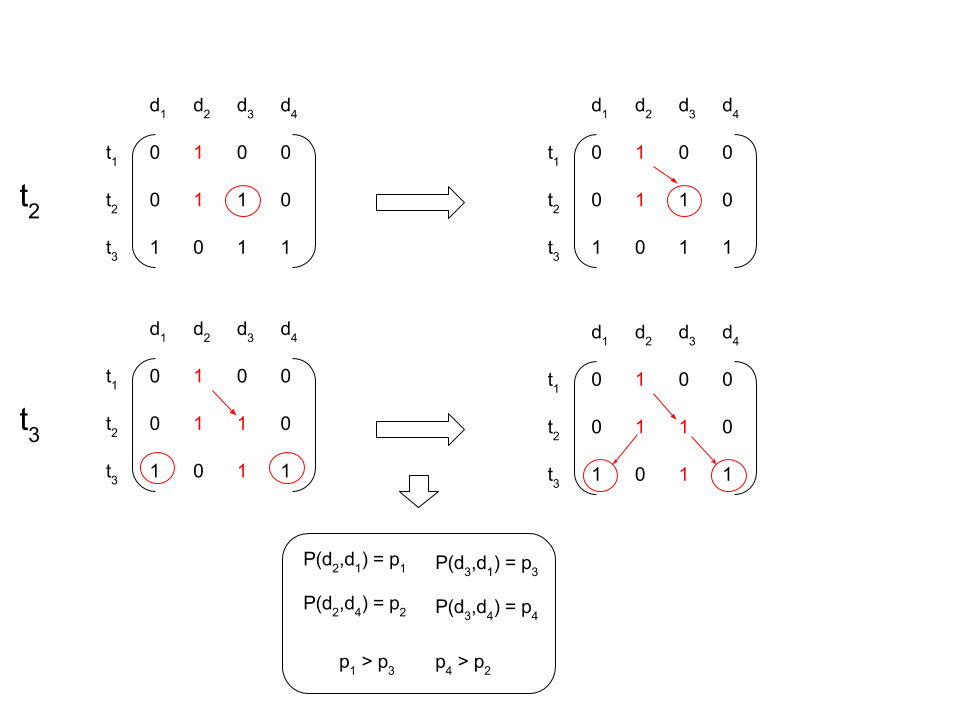
\includegraphics[scale=0.5]{./diagrama1.png}
    % diagrama1.png: 960x720 pixel, 72dpi, 33.87x25.40 cm, bb=0 0 960 720
    \caption{Diagrama Definição de Influência}
  \end{figure}

  Nesse caso, utilizando os valores do exemplo acima, encontramos que o artigo $d_{2}$ influenciou $d_{1}$ e que $d_{3}$ influenciou
  $d_{4}$.
  
  Realizando esse procedimento para cada passo da simulação, construímos a disseminação na rede completa.

  
\pagebreak  
\section{Resultados}
 
Todos os resultados a seguir foram obtidos utilizando o conjunto de dados referente às notícias do atentado ao Charlie Hebdo na mídia
brasileira. 
Esse conjunto de dados contêm 2129 artigos, abaixo temos um gráfico da quantidade de artigos pelo tempo:

\begin{figure}[h]
 \centering
 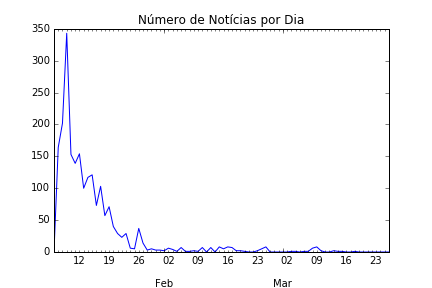
\includegraphics[scale=0.7]{./grafic.png}
 % grafic.png: 432x288 pixel, 72dpi, 15.24x10.16 cm, bb=0 0 432 288
 \caption{Notícias x Tempo}
\end{figure}

Observamos que o crescimento de artigos por tempo dessa notícia foi bem alto durante o mês de janeiro, e que após atingir seu máximo, começou
a cair gradativamente.

\subsection{Rede de Disseminação Real}

Utilizando os dados descritos na seção anterior, construímos a matriz de documentos, que obteve o tamanho 2115x300, onde 2115 são as linhas
que representam cada artigo e o 300 se refere às colunas, que são os atributos definidos pelo modelo \textit{skipgram}.

Podemos observar que o número de artigos na matriz é inferior ao número de artigos totais do conjunto de dados. Isso aconteceu pois 
alguns artigos não obtiveram resultados satisfatórios durante o processo de tokenização, e por isso, foram descartados do conjunto de dados.

Possuindo a matriz de documentos, calculamos então, a matriz de similaridades para podermos construis a rede de disseminação.

\pagebreak
\subsubsection{Definindo Parâmetros}

Após calcular a matriz de documentos e a matriz de similaridades, antes de construir a rede de disseminação,
precisamos definir o tempo máximo de influência de um artigo, e a similaridade de cosseno
mínima para definir se dois artigos são similares. Para isso calculamos a distribuição de cada uma dessas métricas:

\begin{figure}[ht]
 \centering
 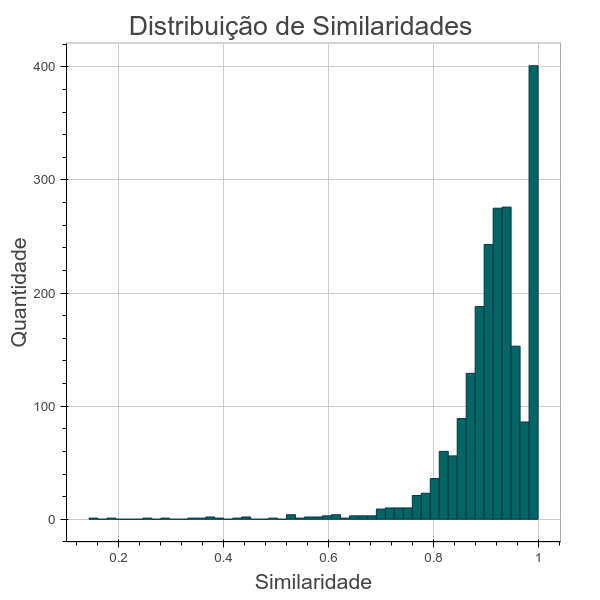
\includegraphics[scale=0.4]{./2.png}
 % 2.png: 600x600 pixel, 72dpi, 21.17x21.17 cm, bb=0 0 600 600
 \caption{Distribuição de Similaridades Máximas}
\end{figure}


Observando as distribuições acima, definimos como similaridade mínima x e tempo máximo de influência de um artigo y.

\pagebreak
\subsubsection{Visualizações da Rede Real}

Utilizando os parâmetros definidos acima, construimos finalmente nossa rede de disseminação do conjunto de dados escolhido.
A rede encontrada possui 1786 vértices, onde cada vértice é um artigo.

Durante a criação da rede, artigos que não possuiam uma relação de influência com nenhum outro foram descartados, o que explica a diferença
do número de nós para o número de artigos presentes na matriz de documentos.

Abaixo temos a distribuição de \textit{out-degrees} da rede:

\begin{figure}[ht]
 \centering
 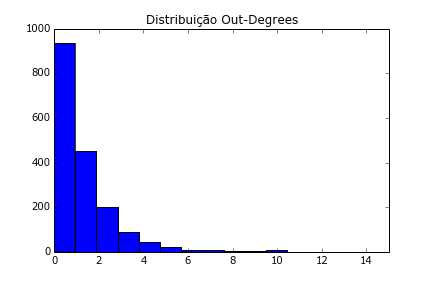
\includegraphics[scale=0.7]{../Notebook/dist_outs.png}
 % dist_outs.png: 432x288 pixel, 72dpi, 15.24x10.16 cm, bb=0 0 432 288
 \caption{Distribuição Out-degrees Rede Real}
\end{figure}

Podemos reparar que, como esperado, possuimos poucos nós com grande grau de influência, isso é, poucos artigos são muito influentes na
mídia. 

Abaixo podemos ver uma visualização da rede criada. Nela, o eixo x representa o passo da infecção, ou seja, os vértices que estão na 
segunda coluna foram influeciados pelos que estão na primeira coluna. Os que estão na terceira coluna foram influenciados pelos da segunda, 
assim sucessivamente. 

O tamanho e cor do vértice indicam o valor do out-degree, quanto maior e mair escuro maior seu out-degree. O mesmo se aplica ao tamanho
do veículo de cada vértice, ou seja, o veículo que publicou o artigo referente ao vértice em questão.

\begin{flushleft}
  \begin{figure}[ht]
  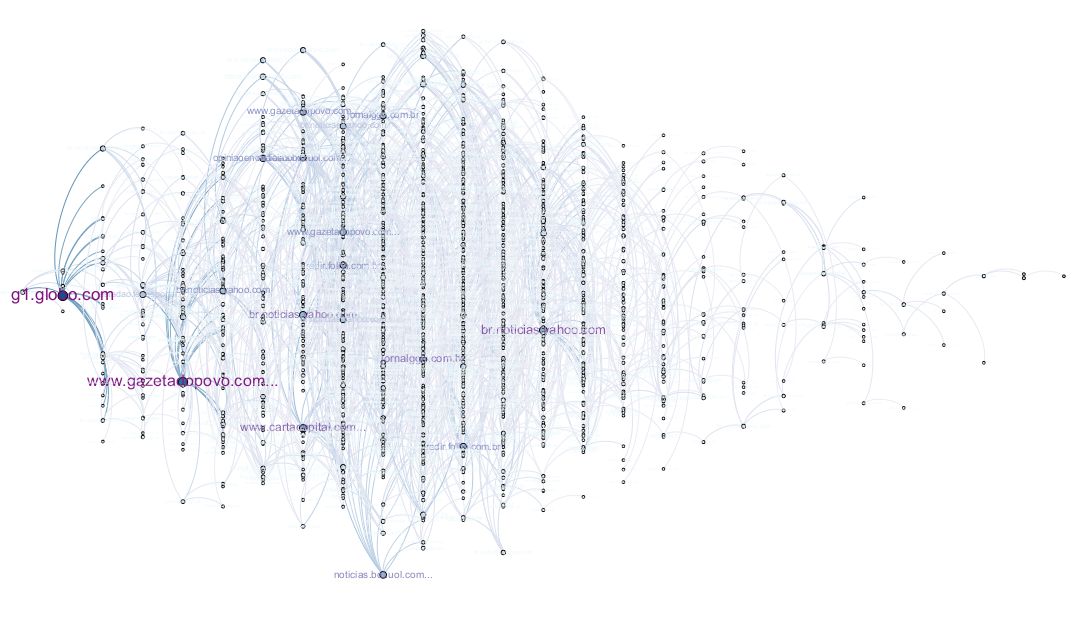
\includegraphics[scale=0.5]{../results/a.png}
  % a.png: 1075x623 pixel, 72dpi, 37.92x21.98 cm, bb=0 0 1075 623
  \caption{Rede Disseminação Real x Passo}
  \end{figure}
\end{flushleft}
\pagebreak

Observando a visualização, vemos que a epidemia acontece rapidamente. Podemos visualizar também alguns veículos como principais influenciadores
em nossa rede, os dois mais influentes são o g1.globo.com e o gazetadopovo.com.br.

Outra forma de visualizar nossa rede é organizar os vértices em função do tempo ao invés do passo de contágio. Abaixo vemos a visualização
onde o eixo x é o tempo, e cada coluna é o tempo $t$ de publicação dos artigos presente nela. Para construir a visualização, definimos
como tempo $t_{0}$ a data de publicação do primeiro artigo publicado. Como espaçar $t$ de hora em hora nos resultou em uma visualização muito confusa,
 resolvemos espaçar de 3 em 3 horas. Dessa forma, na segunda coluna $t_{1}$ encontramos todos os artigos publicados 3 horas após a publicação
 do primeiro artigo, e assim por diante.

Encontramos assim, uma visualização bem longa, com um formato semelhante de um cone deitado. Na medida que o tempo vai passando, nossas
colunas vão diminuindo até não termos mais nenhum artigo. Abaixo mostramos um corte da parte inicial da visualização:

\pagebreak
\begin{figure}[ht]
 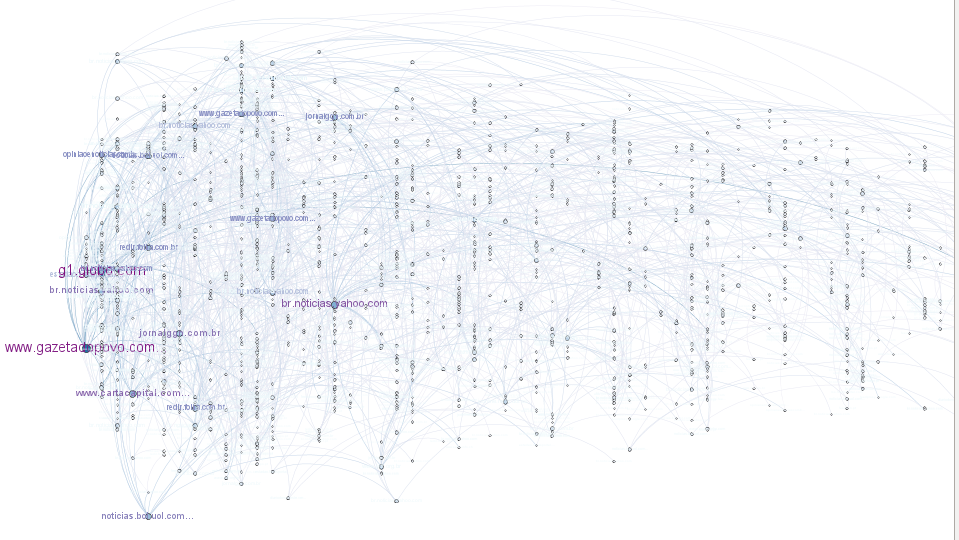
\includegraphics[scale=0.5]{../results/t.png}
 % t.png: 959x540 pixel, 72dpi, 33.83x19.05 cm, bb=0 0 959 540
 \caption{Rede Disseminação Real x Tempo}
\end{figure}

É interessante ver nessa visualização, que os artigos mais influentes se concentram nas primeiras colunas de artigos. Isto é, os artigos que mais
influenciaram sobre a notícia em questão na mídia, foram os publicados bem no início da disseminação.


\subsection{Simulação Rede de Disseminação}

O primeiro passo para a criação da rede simulada, consistia em criar uma rede completa, onde os vértices são os mesmos
da rede real e as arestas são as probabilidades das conexões existirem. Para a construção da rede completa, precisamos
inicialmente das probabilidades de influência entre cada par de veículo presente em nossos dados.

Sendo assim, construímos uma matriz quadrada de probabilidades de influências. A matriz encontrado possui o tamanho 84x84, uma vez que
possuímos 84 veículos responsáveis pela publicação dos artigos de nosso conjunto de dados.

Possuindo a matriz de probabilidades, podemos dar início à construção da rede completa. Realizando as metodologias de construção da matriz
completa, encontramos uma matriz quadrada de tamanho 1786x1786 (número de vértices da rede real). 


\pagebreak
\subsubsection{Resultado Simulação}

Possuingo a matriz de adjacência da rede completa, podemos realizar a simulação do modelo. Porém, precisamos primeiro definir o valor do 
parâmetro $\lambda$. Para definir esse valor, realizamos a simulação para valores variados de lambda, construimos as redes a partir desses
resultados e calculamos a diferença de \textit{Kullback-Leibler}. O $\lambda$ que minimizasse essa diferença, seria o escolhido. Como sabemos
que o $\lambda$ crítico do modelo é dado por:

$$\lambda_{c} = \dfrac{1}{\Lambda}$$

Onde $\Lambda$ é o maior autovalor da matriz de adjacência (\cite{wang2003proceedings}, \cite{chakrabarti2008epidemic}), então testamos
valores próximos ao $\lambda_{c}$. Vemos na tabela
abaixo alguns valores de diferenças encontrados:

\begin{center}
 \begin{tabular}{l|c}
   \ \ \ \ \ $\lambda$ & KL \\ \hline
   $\lambda_{c} + 0.1$ & y\\
   $\lambda_{c} + 0.01$ & 0.014 \\
   $\lambda_{c} + 0.5$ & y
 \end{tabular}
\end{center}

O valor de $\lambda$ que minimizou a diferença de Kullback-Leibler foi $\lambda=0.1$, logo, foi o $\lambda$ utilizado para obter os
resultados a seguir. Abaixo vemos o resultado da simulação feita com 3000 passos e utilizando o parâmetro escolhido:

\begin{figure}[ht]
 \centering
 \includegraphics[scale=0.7]{../data/charlie/simulation.png}
 % simulation.png: 781x584 pixel, 100dpi, 19.84x14.83 cm, bb=0 0 562 420
 \caption{Simulação Modelo}
\end{figure}

Na figura acima possuímos 500 curvas, onde cada curva representa curva de infecção de um artigo. Cada ponto do gráfico diz
respeito à probabilidade do artigo estar infectado no tempo $t$ do modelo. 

O resultado da simulação é um típico resultado para um modelo epidemiológico SIR, o que mostra que nossa matriz de adjacências foi coerente
para a modelagem do sistema e que nossa rede de disseminação real pode ser descrita sim como um processo epidemiológico.

\subsubsection{Rede Simulada}

A simulação do modelo nos retorna uma matriz de estados para cada passo $t$. Utilizando essa matriz, construímos a rede de disseminação simulada.
\subsubsection{Visualizações da Rede Simulada}

\begin{figure}[ht]
 \centering
 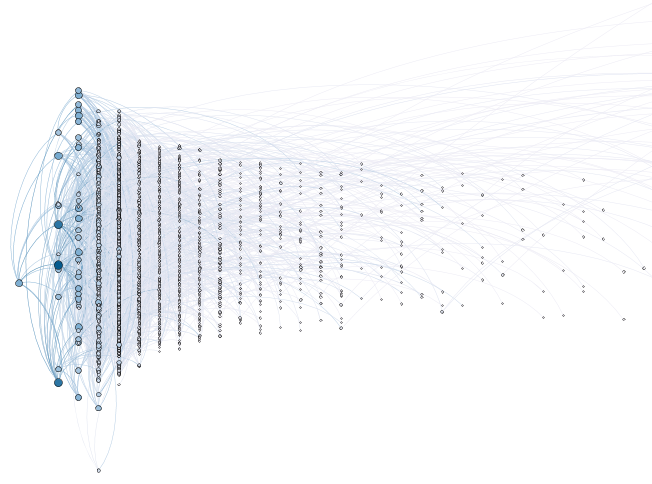
\includegraphics[scale=0.8]{../results/simul.png}
 \caption{Rede Simulada x Tempo}
\end{figure}

\begin{figure}[h]
 \centering
 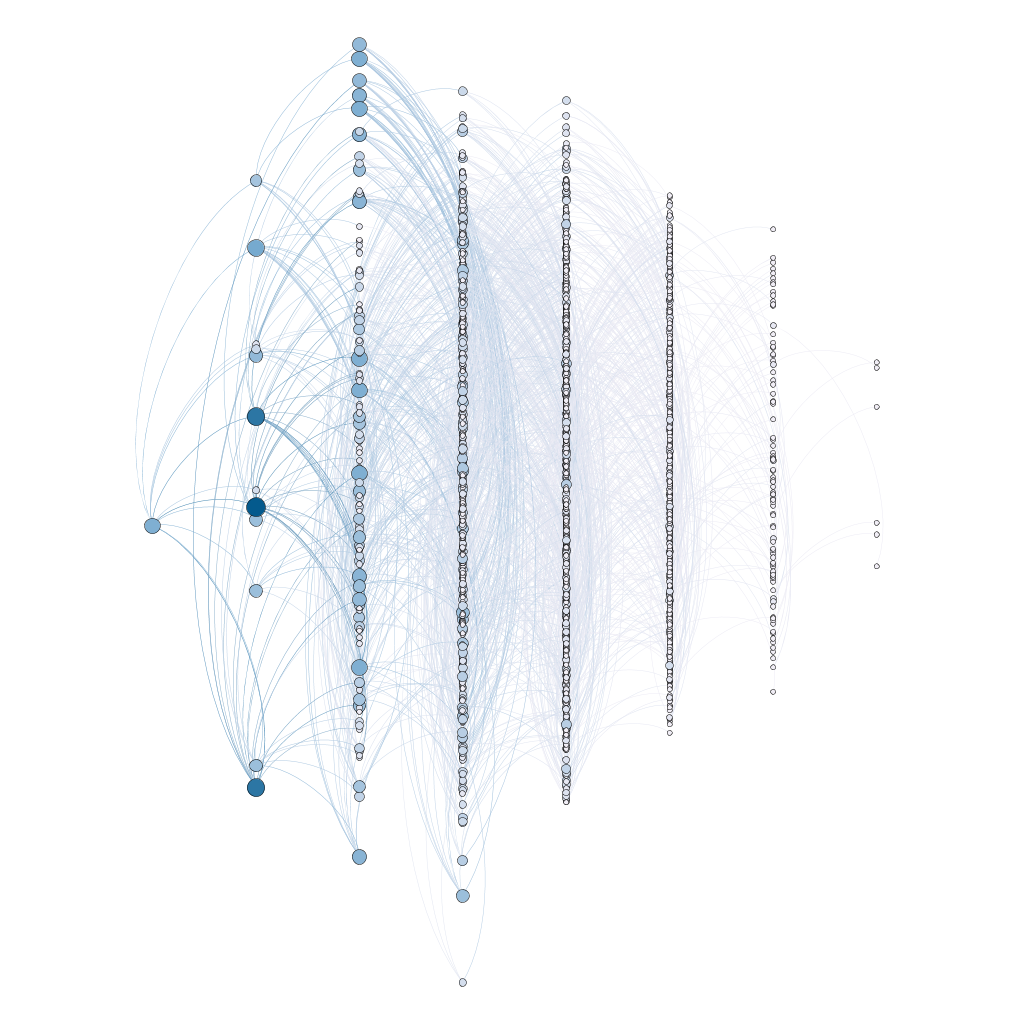
\includegraphics[scale=0.4]{../results/Untitled.png}
 % Untitled.png: 1024x1024 pixel, 72dpi, 36.12x36.12 cm, bb=0 0 1024 1024
 \caption{Rede Simulada x Passo}
\end{figure}




\pagebreak
\section{Conclusão}




\bibliographystyle{plainnat}
\bibliography{ref}
\end{document}
